\cotefile{69}
\scanpage{34}
\mspage{26}
% L1–4
Pour la \inserted{paire de} \deleted{bi}triangles
\figure{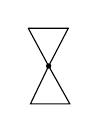
\begin{tikzpicture}[scale=.48]
\draw (-.54,1)--(.52,1)--(0,0)--(-.54,1) (0,0)--(-.48,-1)--(.56,-1)--cycle;
\fill (0,0) circle (2pt);
\end{tikzpicture}}
, \unsure{qu'il|qu'on|quitte} \unsure{faut|peut|à} noter que cette paire ``épinglée'' (pour en éliminer le groupe d'autom. du diagramme, qui est $\mathbb Z/4\mathbb Z$) équivaut :
% L5–8
la \unsure{b.trian|balise} épinglée (en éliminant le groupe d'autom $\mathfrak S_2$ de la \unsure{b.tri.|balise}). \deleted{équivaut : \unsure{la donnée|donc}} \inserted{\unsure{Du pt de vue non}} épinglé : sommet fixé \inserted{$u$}, avec un \unsure{un|ens.} des 2 triangles de sommet $u$, donc

% L9–11
a) un $Q_u$ de cardinal 5, décomposé en $Q'_u$ (de cardinal 2) et $Q''_u$ (de cardinal 3)

b) torseur sous $\Psi(Q_u,\mathbb F_2)=\operatorname{Ker}\bigl(\mathbb F_2^{Q'_u\amalg Q''_u}\longrightarrow\mathbb F_2\bigr)$

% L12–15. The two glosses stand directly underneath their factors.
\uline{Nb} de telles paires
\[
\underset{\substack{\text{sommet}\\u}}{\underline{27}}\cdot
\underset{\substack{\text{partie}\\\text{à 2 él.}\\\text{de }Q_u}}{\binom{5}{2}}
=270=2\cdot3^3\cdot5
\]

Groupe d'autom de $(C,\ \tikz[baseline=-.6ex,scale=.14]{\draw (-1,1.4)--(1,1.4)--(-1,-1.4)--(1,-1.4)--cycle;\fill(0,0) circle (3pt);})$.
\[
\simeq(\unsure{\mathfrak S|\mathfrak G}_2\times\mathfrak S_3)\cdot
\underset{\substack{\unsure{\shortparallel|\cup|\simeq}\\\mathbb F_2^4}}{\Psi(\mathbb F_2)}
\qquad\text{de cardinal }\begin{aligned} &2\cdot6\cdot16\\ &=2^6\cdot3\end{aligned}
\]
% The slant stroke at right links the two numerical lines.
\figure{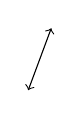
\begin{tikzpicture}[scale=.45]\draw[<->] (0,0)--(.65,1.75);\end{tikzpicture}}
% L16–17
On trouve bien comme produit
\[
2^7\cdot3^4\cdot5=\operatorname{card}W_{E_6}\qquad\ldots
\]
% archive sheet number: 33
